\section{Analyse und Vergleich von Gruppenrichtlinienobjekten }
\subsection{Problemstellung}
    Die Analyse und der Vergleich von Gruppenrichtlinienobjekten (GPOs) in IT-Infrastrukturen stellen eine erhebliche Herausforderung dar, insbesondere bei der Verarbeitung großer Mengen an GPO-Exporten. Die gängigen Exportformate, wie XML und HTML, sind oft schwer interpretierbar und weisen zudem Inkonsistenzen auf. Besonders problematisch sind die Einstellungen im Knoten ExtensionData, da diese heterogenen Strukturen enthalten. Abhängig vom Typ der GPO können hier Skripte, Benutzergruppen, Registrierungswerte oder andere Daten hinterlegt sein, deren Aufbau stark variiert. Diese Vielfalt erschwert eine konsistente und zuverlässige Auswertung erheblich.\newline
    Ein weiteres Problem besteht darin, alle relevanten Eigenschaften der GPOs vollständig und korrekt auszulesen, sowohl für Benutzer- als auch für Computereinstellungen. Unterschiedliche Datenformate und die mangelnde Standardisierung der Exportdaten stellen dabei zusätzliche Hürden dar. 
\subsection{Aufgabenstellung}
    Die Aufgabe besteht darin, ein Konzept zu entwickeln, dass die automatisierte Auswertung und den Vergleich großer Mengen an GPO-Exports möglichst effizient realisiert. Dabei liegt der Schwerpunkt auf der vollständigen und zuverlässigen Erfassung aller relevanten Einstellungen einer GPO, einschließlich der komplexen Extensions Data-Knoten.\newline
    Anschließend soll ein Mechanismus entwickelt werden, der die Unterschiede zwischen den Berichten automatisiert erkennt und darstellt, dazu gehört eine Untersuchung der Eignung der Export Formate XML und HTML hinsichtlich ihrer Effizienz und Konsistenz bei der Verarbeitung. 
\subsection{Grundlagen}
    Für ein klares Verständnis über das Themas sind Grundlagen unerlässlich, deshalb werden anschließend Begriffe erklärt und ihre Bedeutung in Kontext gebracht.
\subsubsection{Gruppenrichtlinienobjekte}
    Gruppenrichtlinienobjekte (GPOs) stellen einen zentralen Bestandteil der IT-Verwaltung innerhalb von Microsoft-basierten Infrastrukturen dar. Sie bestehen aus einer Sammlung definierter Regeln, mit deren Hilfe sich das Verhalten von Computern und Benutzerkonten im Netzwerk zentral steuern und standardisieren lässt. Die Konfiguration und Verwaltung dieser Objekte erfolgt über die Gruppenrichtlinienverwaltungs-Konsole (Group Policy Management Console, GPMC), die als zentrales Werkzeug zur Strukturierung und Kontrolle von Richtlinieneinstellungen dient \cite{orin-thomas_group_nodate}. 
\subsubsection{Gruppenrichtlinienverwaltungs-Konsole (GPMC)}
    Die Group Policy Management Console (GPMC) stellt ein zentrales Verwaltungswerkzeug dar, das in Microsoft-Umgebungen zur strukturierten Organisation und Steuerung von Gruppenrichtlinien eingesetzt wird. Sie ermöglicht eine zentrale Sicht auf alle GPOs innerhalb einer Active-Directory-Infrastruktur und vereinfacht deren Handhabung durch eine einheitliche Benutzeroberfläche.\newline
    Über die GPMC lassen sich Richtlinien zielgerichtet auf einzelne Organisationseinheiten, Standorte oder ganze Domänen anwenden. Zudem bietet sie Funktionen zur Priorisierung, Vererbungsanalyse und Konfliktauflösung, wodurch eine transparente Richtlinienverwaltung über verschiedene Ebenen hinweg realisierbar wird.
    Ein weiterer zentraler Bestandteil ist die Möglichkeit, Richtlinieninhalte in verschiedenen Formaten zu exportieren. Insbesondere die Ausgabe als XML oder HTML spielt im Rahmen dieser Arbeit eine wichtige Rolle, da sie die Grundlage für den automatisierten Vergleich der GPO-Inhalte bildet \cite{orin-thomas_group_nodate-1}. 
\subsection{Analyse bestehender Methoden}
    Zur Identifikation geeigneter Verfahren für den Vergleich von Gruppenrichtlinienobjekten wurden zunächst bestehende Ansätze aus der Praxis und gängige Werkzeuge untersucht. Ziel war es, herauszufinden, inwieweit diese Ansätze die Anforderungen an Vollständigkeit, Skalierbarkeit und Automatisierbarkeit erfüllen.\newline
    Ein häufiger Ansatz ist der manuelle Vergleich über die Gruppenrichtlinien-verwaltungs-Konsole (GPMC), bei dem einzelne GPOs visuell miteinander ab-geglichen werden. Dieser Weg ist in kleinen Umgebungen mit wenigen GPOs prinzipiell umsetzbar, skaliert jedoch schlecht. Zudem besteht ein hohes Risiko, Änderungen zu übersehen, insbesondere bei umfangreichen oder komplex verschachtelten Richtlinien.\newline
    Verschiedene Drittanbietertools bieten zum Teil integrierte Vergleichsfunktionen, jedoch häufig mit Einschränkungen bei Transparenz, Anpassbarkeit oder Lizenzierung. In vielen Fällen sind diese Lösungen nicht flexibel genug, um auf spezifische Anforderungen oder bestehende Automatisierungsprozesse einzugehen.\newline
    Für die vorliegende Aufgabenstellung war daher ein eigener Lösungsansatz erforderlich, der unabhängig von kommerziellen Tools arbeitet, sich leicht in bestehende Prozesse integrieren lässt und eine hohe Nachvollziehbarkeit der Ergebnisse ermöglicht. Dabei stand die automatisierte Verarbeitung der GPO-Daten im Mittelpunkt – insbesondere im Hinblick auf deren Export aus der GPMC. Die Frage nach dem geeigneten Exportformat spielte hierbei eine zentrale Rolle und wird im folgenden Kapitel detailliert betrachtet. 
\subsection{Vergleich der Exportformate: HTML vs. XML }
    Im Rahmen der Konzeptentwicklung war die Wahl des geeigneten Exportformats ein entscheidender Faktor für die Realisierbarkeit einer automatisierten Vergleichsmethode. Die Gruppenrichtlinienverwaltungs-Konsole (GPMC) stellt standardmäßig zwei Formate für den Export von GPO-Berichten zur Verfügung: HTML und XML. Beide Formate enthalten im Wesentlichen dieselben Informationen, unterscheiden sich jedoch grundlegend in Struktur, Zweck und Verarbeitbarkeit. Die folgende Tabelle zeigt die wichtigsten Unterschiede zwischen beiden Formaten im direkten Vergleich.
    \begin{table}[H]
\centering
\renewcommand{\arraystretch}{1.3} % etwas mehr Zeilenhöhe
\begin{tabularx}{\textwidth}{@{}p{3.5cm}Xp{3.5cm}@{}}
\toprule
\textbf{Kriterium} & \textbf{HTML} & \textbf{XML} \\
\midrule
Zielgruppe & Menschliche Leser, Administratoren & Automatisierte Systeme, Skripte \\
Lesbarkeit & Hoch – gut formatiert, direkt im Browser darstellbar & Gering, primär maschinenlesbar \\
Visualisierung & Unterstützt Diagramme & Keine grafische Aufbereitung \\
Verarbeitung per Skript & Eingeschränkt & Sehr gut, klar strukturiert \\
Konsistenz bei Änderungen & Niedrig & Hoch \\
Dateigröße und Performance & Kann bei vielen Elementen groß werden und langsam sein & Kompakter und performanter \\
Flexibilität der Weiterverarbeitung & Eingeschränkt & Hoch \\
Erstellungsmöglichkeiten der Berichte & Direkt über GPMC & Über GPMC oder PowerShell \\
\bottomrule
\end{tabularx}
\caption{Vergleich von HTML- und XML-Eigenschaften im Kontext von Berichten}
\label{tab:html-vs-xml}
\end{table}
Das HTML-Format ist primär auf die visuelle Darstellung für den Administrator ausgelegt. Informationen werden in einer formatierten, aber nicht standardisierten Struktur bereitgestellt. Für die manuelle Durchsicht oder den Einsatz in Dokumentationen ist dieses Format geeignet, stößt jedoch bei der automatisierten Weiterverarbeitung schnell an Grenzen. Die semantische Struktur fehlt weitgehend, was eine zuverlässige Extraktion einzelner Einstellungen erschwert und den Einsatz robuster Parsing\footnote{„Parsen“ bedeutet, dass ein Programm den Text analysiert und in seine logischen Bestandteile zerlegt, um die Struktur und Inhalte maschinell weiterzuverarbeiten.}-Methoden erforderlich macht. Bereits geringfügige Änderungen am Layout oder am HTML-Markup können bestehende Skripte unbrauchbar machen.\newline
Das XML-Format hingegen ist speziell für die strukturierte und maschinenlesbare Repräsentation konzipiert. Jeder relevante Abschnitt einer GPO ist durch klar definierte Tags gekennzeichnet. Insbesondere komplexe Knoten wie ExtensionsData lassen sich gezielt ansprechen und extrahieren, ohne auf visuelle Merkmale angewiesen zu sein. Diese Eigenschaften machten XML zur bevorzugten Wahl für eine automatisierte Auswertung und einen systematischen Vergleich von GPOs. 
\newpage
\subsection{Konzeptentwicklung}
    Die Entwicklung eines effizienten und praxistauglichen Konzepts zum automatisierten Vergleich von Gruppenrichtlinien stand im Mittelpunkt der Praxisphase. Im Folgenden werden die Zielsetzung, die Evaluationskriterien sowie die begründete Entscheidung für XML als Exportformat und Excel als Vergleichsplattform detailliert erläutert. 
\subsubsection{Zielsetzung des Konzepts}
    Das primäre Ziel bestand darin, eine reproduzierbare und skalierbare Methode zu entwickeln, um Unterschiede zwischen zwei Gruppenrichtlinienobjekten (GPOs) automatisiert zu identifizieren. Dabei sollten folgende Anforderungen erfüllt werden:\newline
    1. Reduktion manueller Arbeitsschritte: Beseitigung zeitintensiver, fehleranfälliger manueller Vergleiche.\newline
    2. Standardisierung: Schaffung eines einheitlichen Prozesses für zukünftige GPO-Audits.\newline
    3. Integration in bestehende Prozesse: Nahtlose Einbindung in die Microsoft-basierte IT-Infrastruktur des Unternehmens. 
\subsubsection{Kriterien für die Auswahl der Methode}
    Die Konzeption der Lösung basierte auf drei zentralen Anforderungen, die den gesamten Entwicklungsprozess maßgeblich prägten.\newline
    Erstens stand die Automatisierbarkeit im Fokus: Die Lösung sollte in der Lage sein, Differenzen zwischen den Datensätzen vollständig ohne manuelle Eingriffe zu erkennen und zu protokollieren. Zweitens wurde besonderes Augenmerk auf die Lesbarkeit der Ergebnisse gelegt – sowohl für technische als auch für fachliche Nutzergruppen mussten die Auswertungen klar nachvollziehbar und verständlich aufbereitet sein. Drittens wurde eine hohe Vergleichbarkeit angestrebt, wobei nicht nur inhaltliche Abweichungen, sondern auch strukturelle Unterschiede – etwa bei verschachtelten Richtlinienparametern – zuverlässig erfasst werden sollten.\newline
    Ergänzend dazu waren auch die Kompatibilität mit der bestehenden Unternehmensinfrastruktur sowie ein möglichst geringer Wartungsaufwand ausschlaggebend für die Auswahl und Ausgestaltung der eingesetzten Methoden und Werkzeuge.
\subsubsection{Begründete Entscheidung für Excel}
    Für die Gegenüberstellung der extrahierten GPO-Daten wurde eine Excel-basierte Lösung eingesetzt, da sie sowohl funktional als auch wirtschaftlich überzeugte. Zwar wurden alternative Vergleichstools wie WinMerge, Altova DiffDog und Beyond Compare evaluiert, jedoch letztlich verworfen.\newline WinMerge bietet als Open-Source-Anwendung zwar grundlegende Funktionen zum Textvergleich, benötigt für den Einsatz mit Excel-Dateien jedoch zusätzliche Plugins, was die Komplexität erhöhte und potenzielle Stabilitätsprobleme mit sich brachte. Altova DiffDog und Beyond Compare überzeugten zwar durch ihre leistungsstarke Analyse von strukturierten Daten wie XML oder Excel, waren jedoch aufgrund fehlender Unternehmenslizenzen nicht einsetzbar, da beide Programme kostenpflichtig sind.\newline
    Im Gegensatz dazu bot Microsoft Excel mehrere entscheidende Vorteile: Durch vorhandene Volumenlizenzen konnte es kostenfrei genutzt werden, ohne zusätzlichen finanziellen Aufwand. Zudem war Excel in der IT-Abteilung bereits als Standardwerkzeug für Berichte etabliert, sodass keine Einarbeitungszeit erforderlich war. Ein weiterer zentraler Aspekt war die Flexibilität durch VBA, die es ermöglichte, individuelle Vergleichslogiken zu implementieren. Die tabellarische Struktur von Excel erlaubte darüber hinaus die Nutzung von Sortier- und Filterfunktionen, wodurch selbst komplexe GPO-Hierarchien übersichtlich dargestellt werden konnten.\newline
    Die Lösung ermöglichte eine End-to-End-Integration: Vom Export der XML-Dateien über die Transformation der Rohdaten mittels PowerShell bis hin zur differenzierenden Auswertung der Einstellungsparameter wurde der gesamte Prozess in Excel konsolidiert. So wurden beispielsweise die extrahierten XML-Daten der GPOs aus der Kunden- und der Referenzumgebung in getrennte Arbeitsblätter geladen. Ein darauf abgestimmtes VBA-Skript führte anschließend einen zeilenweisen Abgleich der Parameter durch und markierte Abweichungen automatisch. Dadurch ließ sich der manuelle Analyseaufwand erheblich reduzieren – von mehreren Stunden auf wenige Minuten.
\subsection{Technische Umsetzung}
    Die technische Realisierung des automatisierten GPO-Vergleichs umfasste mehrere aufeinander aufbauende Schritte, die von der Datenextraktion bis zur differenzierten Auswertung reichten. Die Umsetzung basierte auf einer Kombination aus bestehenden Skripten, Anpassungen an die Projektanforderungen und der Entwicklung neuer Automatisierungslösungen.
\subsubsection{Workflow-Übersicht}
    Der gesamte Prozess gliederte sich in mehrere aufeinanderfolgenden Phasen, die eine strukturierte und reproduzierbare Durchführung ermöglichten. Zu Beginn des Projekts erfolgte die Bereitstellung einer Testumgebung in Form einer virtuellen Maschine mit vorkonfigurierten Gruppenrichtlinien. Diese Umgebung diente als Referenzbasis, um die geplante Vergleichsmethodik unter kontrollierten Bedingungen zu entwickeln und zu validieren.\newline 
    Darauf folgend wurden die Gruppenrichtlinienobjekte (GPOs) sowohl der Ziel- als auch der Referenzumgebung über die Group Policy Management Console (GPMC) als XML-Dateien exportiert. Diese Dateien enthielten sämtliche Richtlinieneinstellungen in strukturierter Form und bildeten die Grundlage für die nachfolgende Verarbeitung.\newline
    Für das Parsing und die Vorverarbeitung der XML-Daten kam ein von P. Dosch bereitgestelltes PowerShell-Skript zum Einsatz. Dieses extrahierte gezielt die relevanten Einstellungen, filterte irrelevante Metadaten heraus und überführte die Informationen in ein tabellarisches Format.\newline 
    Die so aufbereiteten Daten wurden in zwei separate Excel-Tabellen überführt – jeweils eine für die Kundenumgebung und eine für die Referenzkonfiguration. Darauf aufbauend erfolgte der automatisierte Vergleich durch ein speziell entwickeltes VBA-Skript, das beide Tabellen zeilenweise analysierte, Abweichungen identifizierte und diese in einer separaten Auswertungstabelle mit visueller Hervorhebung dokumentierte.
\subsubsection{Anpassung des bestehenden PowerShell-Skripts}
    Das ursprünglich von P. Dosch entwickelte PowerShell-Skript bildete die technische Grundlage für die XML-Verarbeitung, musste jedoch im Verlauf des Projekts an die spezifischen Anforderungen angepasst werden. Eine zentrale Erweiterung betraf die selektive Datenextraktion: Hierzu wurden zusätzliche XPath-Abfragen implementiert, um gezielt auch komplex verschachtelte Konfigurationen – etwa innerhalb des Knotens ExtensionsData - RegistrySettings auszulesen. Diese Strukturen waren im ursprünglichen Skript nicht berücksichtigt worden, jedoch für die Vergleichsanalyse essenziell.\newline 
    Darüber hinaus wurde die Standardisierung der Ausgabestruktur überarbeitet, um eine einheitliche Spaltenreihenfolge in den resultierenden Excel-Dateien sicherzustellen. Diese Maßnahme war erforderlich, um die Vergleichbarkeit der Datensätze im weiteren Verlauf automatisiert gewährleisten zu können. Ergänzend wurde die bestehende Skriptlogik durch robuste Fehlerbehandlungsmechanismen erweitert. Durch die Integration von Try-Catch-Blöcken konnten potenzielle Probleme - etwa fehlerhafte XML-Syntax oder fehlende Datenknoten - gezielt abgefangen und in einem separaten Logfile dokumentiert werden, ohne den gesamten Verarbeitungsprozess zu unterbrechen.
\subsubsection{Entwicklung der Excel-VBA-Lösung}
    Der Grundbaustein der Automatisierung bildete ein in Excel integriertes VBA-Makro, das mehrere zentrale Funktionen übernahm. Zunächst erfolgte der Datenimport beider Vergleichstabellen in den Arbeitsspeicher, gefolgt von einer Validierung der Spaltenüberschriften. Bei Unstimmigkeiten wurde der Prozess kontrolliert abgebrochen und durch eine Fehlermeldung signalisiert. Die eigentliche Vergleichslogik basierte auf einem zeilenweisen Abgleich eindeutiger Schlüsselwerte - beispielsweise der Kombination aus Einstellungsname und Status. Abweichungen in den Einstellungswerten, etwa zwischen aktivierten und deaktivierten Optionen oder bei unterschiedlichen Namen, wurden systematisch in einer separaten Differenztabelle dokumentiert. Zur besseren Nachvollziehbarkeit kamen zudem visuelle Hervorhebungen mittels bedingter Formatierung zum Einsatz: Fehlende Einträge wurden rot, abweichende Werte gelb markiert.\begin{figure}[H]
    \centering
    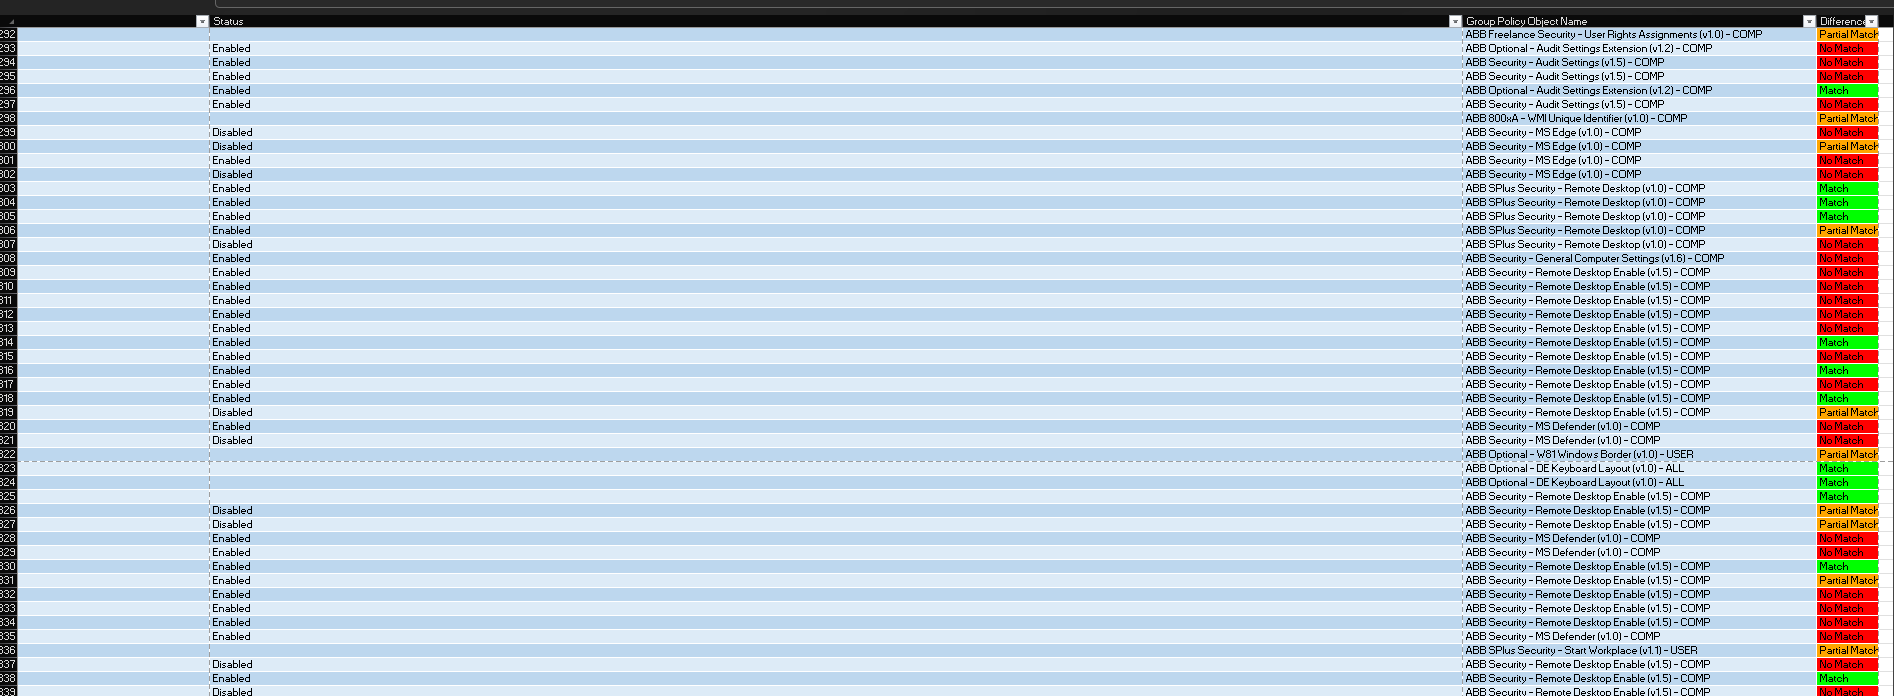
\includegraphics[width=1\textwidth]{IMG/Screenshot 2025-03-21 070630.png}
    \caption{Erzeugte Excel Tabelle mit Farblicher Hervorhebung der Unterschiede}
    \end{figure}
    \label{Excel Ergebniss Tabelle} Ergänzend erstellte das Skript einen Zusammenfassungsbericht, der eine statistische Übersicht über die Anzahl und Art der Unterschiede bot.
    \begin{figure}[H]
    \centering
    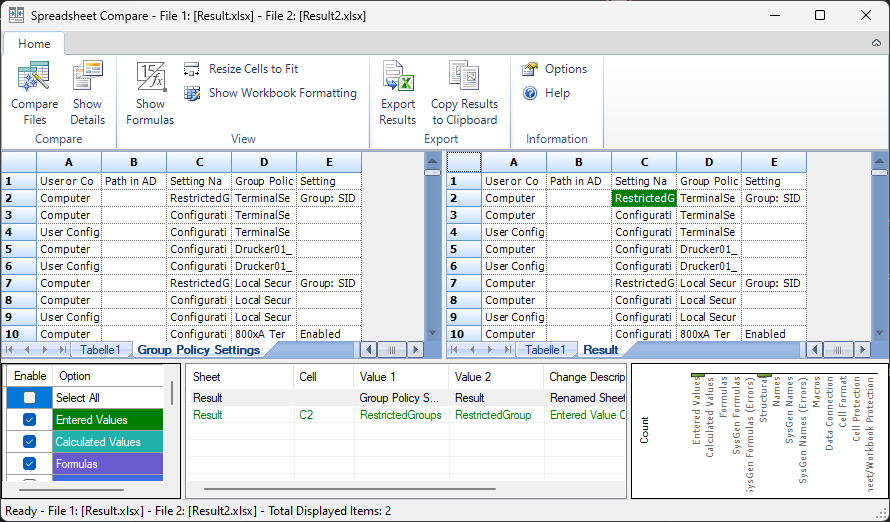
\includegraphics[width=1\textwidth]{IMG/Screenshot 2025-02-18 110333.png}
    \caption{Zusammenfassung der Unterschiede im separaten Dokument}
    \label{Zusammengefaste darstellung des vergleichs}
    \end{figure}
    Abschließend ermöglichte eine integrierte Exportfunktion das Speichern der Differenztabelle im CSV- oder PDF-Format, wodurch die Ergebnisse beispielsweise für Audits oder Besprechungen zur Verfügung gestellt werden konnten.
\subsubsection{Eingesetzte Tools und Technologien}
    Zur Umsetzung des Projekts kamen verschiedene Werkzeuge zum Einsatz, die jeweils spezifische Aufgabenbereiche abdeckten. Die Verarbeitung der XML-Dateien, einschließlich der Filterung relevanter Einstellungen sowie der Generierung von CSV-Rohdaten diente Powershell 7.2 als zentrale Plattform für die anschließende Datentransformation, den Abgleich der Werte und deren Visualisierung diente Microsoft Excel 365. Die in Excel integrierte Programmiersprache VBA wurde zur Umsetzung der Vergleichslogik sowie zur Erstellung einer benutzerfreundlichen Oberfläche verwendet - beispielsweise durch Schaltflächen zum Starten des Vergleichsprozesses. Für das effiziente Einlesen und Interpretieren der umfangreichen XML-Datenstrukturen kamen zudem die .NET-basierten System.Xml-Module von PowerShell zum Einsatz.
    Die entwickelte Lösung lässt sich in folgenden Bereichen weiter optimieren: 
\begin{itemize}
    \item Scheduled Tasks: 
    Durch die Anbindung an Windows-Aufgabenplanung könnte der gesamte Workflow (Export → Parsing → Vergleich) täglich oder wöchentlich automatisiert ausgeführt werden.
    \item Erweiterte Analysen:
    Die VBA-Logik könnte um Machine-Learning-Module ergänzt werden, um historische Änderungsmuster zu erkennen und Risikoabschätzungen vorzunehmen. 
\end{itemize}
\subsection{Fazit des ersten Praxiseinsatzes und Ausblick}
Im Rahmen dieses Projekts wurde ein Vergleichstool zur Analyse von Gruppenrichtlinieneinstellungen (GPOs) zwischen Kundensystemen und dem unternehmenseigenen Standard entwickelt. Die Rohdaten wurden dabei aus XML-Dokumenten extrahiert, da dieses Format aufgrund seiner strukturierten Natur zunächst als besonders geeignet erschien.\newline
Im Verlauf der Umsetzung zeigte sich jedoch, dass die XML-Daten nicht durchgängig konsistent strukturiert waren. Einzelne Einstellungen wurden uneinheitlich dargestellt, was zu fehlerhaften Auslesungen führte und die automatische Übertragung in die Vergleichstabelle erschwerte. Dies wirkte sich direkt auf die Genauigkeit des VBA-basierten Vergleichsskripts aus, das auf eine saubere Datenbasis angewiesen ist.\newline 
Diese Erkenntnis legt nahe, dass HTML-Dokumente trotz ihrer vermeintlich geringeren Strukturierung unter bestimmten Bedingungen eine verlässlichere Datenquelle darstellen können. Durch eine gezielte Anpassung des PowerShell-Skripts wäre es möglich, HTML-Dokumente nach relevanten Informationen zu filtern und so eine konsistentere Datenbasis für den Vergleich zu schaffen.\newline
Für zukünftige Projekte empfiehlt sich daher eine frühzeitige Validierung der Datenquellen hinsichtlich ihrer Struktur und Konsistenz. Zudem kann eine modulare Erweiterung des Tools um eine alternative HTML-Auslesung die Flexibilität und Robustheit der Lösung deutlich erhöhen. Ein weiterführender Ansatz ist die Entwicklung eines hybriden Parsers, der je nach Datenqualität zwischen XML und HTML wechseln kann.